\documentclass{standalone}
\usepackage{tikz}
\usetikzlibrary{patterns, positioning}

\begin{document}
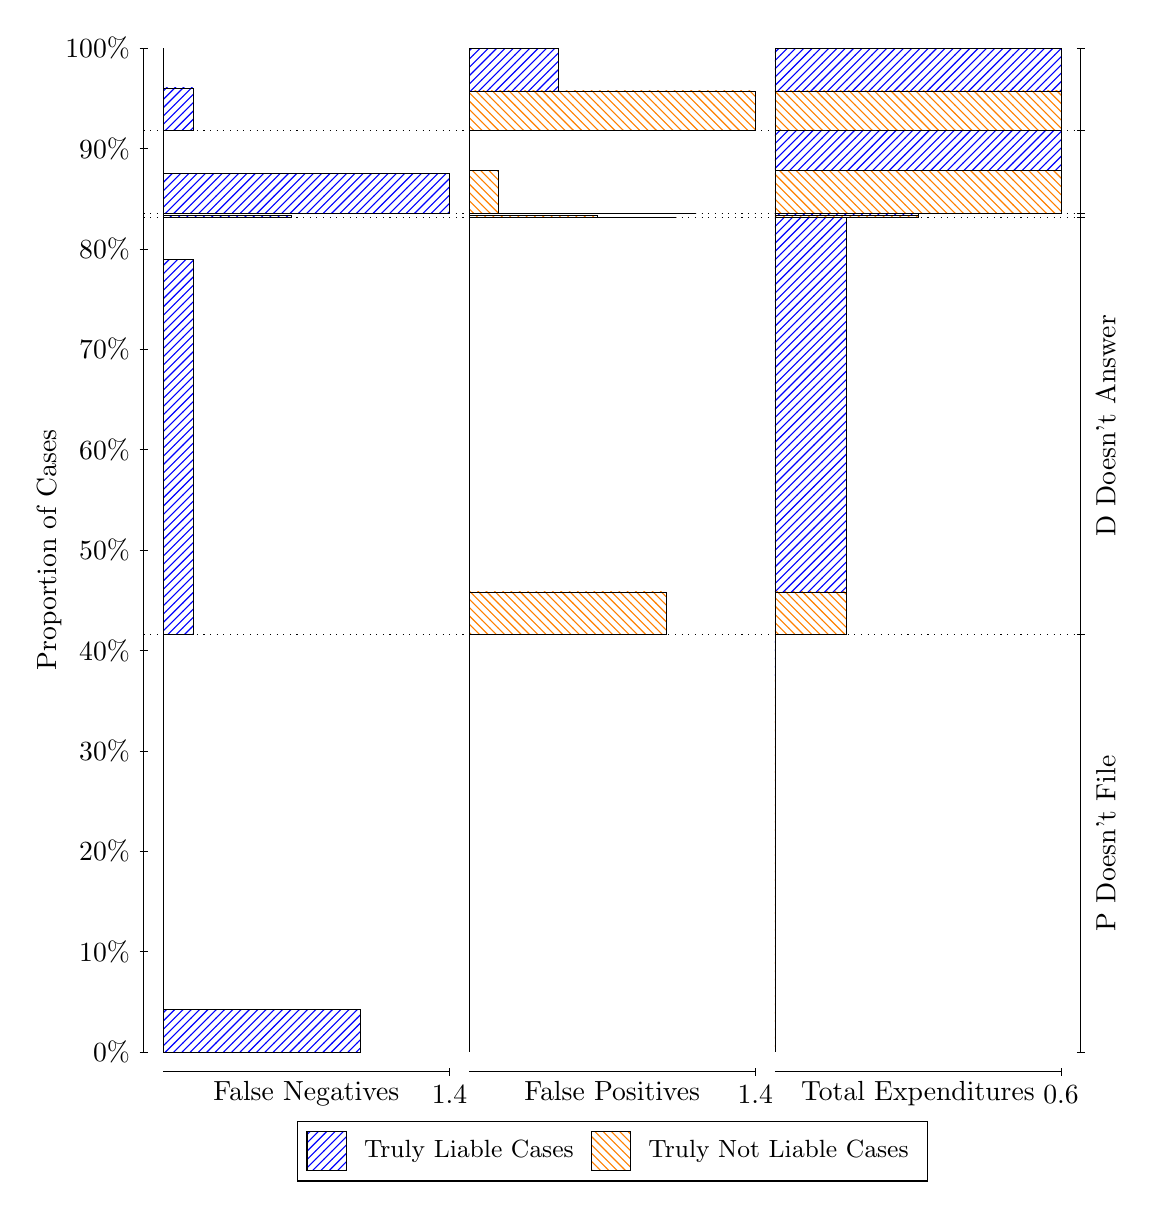
\begin{tikzpicture}
\draw[black, very thin] (1.5,1.75) -- (1.5,14.5);
\node[rotate=90, anchor=center] at (0.3, 8.125) {Proportion of Cases};
\draw[black, very thin] (1.45,1.75) -- (1.55,1.75);
\node[anchor=east] at (1.45, 1.75) {0\%};
\draw[black, very thin] (1.45,3.025) -- (1.55,3.025);
\node[anchor=east] at (1.45, 3.025) {10\%};
\draw[black, very thin] (1.45,4.3) -- (1.55,4.3);
\node[anchor=east] at (1.45, 4.3) {20\%};
\draw[black, very thin] (1.45,5.575) -- (1.55,5.575);
\node[anchor=east] at (1.45, 5.575) {30\%};
\draw[black, very thin] (1.45,6.85) -- (1.55,6.85);
\node[anchor=east] at (1.45, 6.85) {40\%};
\draw[black, very thin] (1.45,8.125) -- (1.55,8.125);
\node[anchor=east] at (1.45, 8.125) {50\%};
\draw[black, very thin] (1.45,9.4) -- (1.55,9.4);
\node[anchor=east] at (1.45, 9.4) {60\%};
\draw[black, very thin] (1.45,10.675) -- (1.55,10.675);
\node[anchor=east] at (1.45, 10.675) {70\%};
\draw[black, very thin] (1.45,11.95) -- (1.55,11.95);
\node[anchor=east] at (1.45, 11.95) {80\%};
\draw[black, very thin] (1.45,13.225) -- (1.55,13.225);
\node[anchor=east] at (1.45, 13.225) {90\%};
\draw[black, very thin] (1.45,14.5) -- (1.55,14.5);
\node[anchor=east] at (1.45, 14.5) {100\%};

\draw[black, very thin] (13.4,1.75) -- (13.4,14.5);
\draw[black, very thin] (13.35,1.75) -- (13.45,1.75);
\node[anchor=west] at (13.35, 1.75) {};
\draw[black, very thin] (13.35,7.0516) -- (13.45,7.0516);
\node[anchor=west] at (13.35, 7.0516) {};
\draw[black, very thin] (13.35,12.352) -- (13.45,12.352);
\node[anchor=west] at (13.35, 12.352) {};
\draw[black, very thin] (13.35,12.401) -- (13.45,12.401);
\node[anchor=west] at (13.35, 12.401) {};
\draw[black, very thin] (13.35,12.401) -- (13.45,12.401);
\node[anchor=west] at (13.35, 12.401) {};
\draw[black, very thin] (13.35,13.45) -- (13.45,13.45);
\node[anchor=west] at (13.35, 13.45) {};
\draw[black, very thin] (13.35,14.5) -- (13.45,14.5);
\node[anchor=west] at (13.35, 14.5) {};

\draw[black, very thin, pattern color=blue, pattern=north east lines] (1.75,1.75) rectangle (4.2557,2.2912);
\draw[black, very thin, pattern color=orange, pattern=north west lines] (1.75,2.2912) rectangle (1.75,7.0516);
\draw[black, very thin, pattern color=blue, pattern=north east lines] (1.75,7.0516) rectangle (2.1259,11.811);
\draw[black, very thin, pattern color=orange, pattern=north west lines] (1.75,11.811) rectangle (1.75,12.352);
\draw[black, very thin, pattern color=blue, pattern=north east lines] (1.75,12.352) rectangle (3.3787,12.376);
\draw[black, very thin, pattern color=blue, pattern=north east lines] (1.75,12.376) rectangle (3.1282,12.376);
\draw[black, very thin, pattern color=blue, pattern=north east lines] (1.75,12.376) rectangle (2.8776,12.376);
\draw[black, very thin, pattern color=blue, pattern=north east lines] (1.75,12.376) rectangle (2.627,12.376);
\draw[black, very thin, pattern color=blue, pattern=north east lines] (1.75,12.376) rectangle (2.3764,12.376);
\draw[black, very thin, pattern color=orange, pattern=north west lines] (1.75,12.376) rectangle (1.75,12.401);
\draw[black, very thin, pattern color=blue, pattern=north east lines] (1.75,12.401) rectangle (2.1259,12.401);
\draw[black, very thin, pattern color=orange, pattern=north west lines] (1.75,12.401) rectangle (1.75,12.401);
\draw[black, very thin, pattern color=blue, pattern=north east lines] (1.75,12.401) rectangle (5.3833,12.907);
\draw[black, very thin, pattern color=orange, pattern=north west lines] (1.75,12.907) rectangle (1.75,13.45);
\draw[black, very thin, pattern color=blue, pattern=north east lines] (1.75,13.45) rectangle (2.1259,13.993);
\draw[black, very thin, pattern color=orange, pattern=north west lines] (1.75,13.993) rectangle (1.75,14.5);
\draw[black, very thin, pattern color=orange, pattern=north west lines] (5.6333,1.75) rectangle (5.6333,6.5104);
\draw[black, very thin, pattern color=blue, pattern=north east lines] (5.6333,6.5104) rectangle (5.6333,7.0516);
\draw[black, very thin, pattern color=orange, pattern=north west lines] (5.6333,7.0516) rectangle (8.1391,7.5922);
\draw[black, very thin, pattern color=blue, pattern=north east lines] (5.6333,7.5922) rectangle (5.6333,12.352);
\draw[black, very thin, pattern color=orange, pattern=north west lines] (5.6333,12.352) rectangle (8.2644,12.352);
\draw[black, very thin, pattern color=orange, pattern=north west lines] (5.6333,12.352) rectangle (8.0138,12.352);
\draw[black, very thin, pattern color=orange, pattern=north west lines] (5.6333,12.352) rectangle (7.7632,12.352);
\draw[black, very thin, pattern color=orange, pattern=north west lines] (5.6333,12.352) rectangle (7.5126,12.352);
\draw[black, very thin, pattern color=orange, pattern=north west lines] (5.6333,12.352) rectangle (7.2621,12.376);
\draw[black, very thin, pattern color=blue, pattern=north east lines] (5.6333,12.376) rectangle (5.7586,12.376);
\draw[black, very thin, pattern color=blue, pattern=north east lines] (5.6333,12.376) rectangle (5.6333,12.401);
\draw[black, very thin, pattern color=orange, pattern=north west lines] (5.6333,12.401) rectangle (8.5149,12.401);
\draw[black, very thin, pattern color=blue, pattern=north east lines] (5.6333,12.401) rectangle (6.0092,12.401);
\draw[black, very thin, pattern color=orange, pattern=north west lines] (5.6333,12.401) rectangle (6.0092,12.944);
\draw[black, very thin, pattern color=blue, pattern=north east lines] (5.6333,12.944) rectangle (5.6333,13.45);
\draw[black, very thin, pattern color=orange, pattern=north west lines] (5.6333,13.45) rectangle (9.2667,13.957);
\draw[black, very thin, pattern color=blue, pattern=north east lines] (5.6333,13.957) rectangle (6.7609,14.5);
\draw[black, very thin, pattern color=orange, pattern=north west lines] (9.5167,1.75) rectangle (9.5167,6.5104);
\draw[black, very thin, pattern color=blue, pattern=north east lines] (9.5167,6.5104) rectangle (9.5167,7.0516);
\draw[black, very thin, pattern color=orange, pattern=north west lines] (9.5167,7.0516) rectangle (10.425,7.5922);
\draw[black, very thin, pattern color=blue, pattern=north east lines] (9.5167,7.5922) rectangle (10.425,12.352);
\draw[black, very thin, pattern color=orange, pattern=north west lines] (9.5167,12.352) rectangle (11.333,12.376);
\draw[black, very thin, pattern color=blue, pattern=north east lines] (9.5167,12.376) rectangle (11.333,12.401);
\draw[black, very thin, pattern color=orange, pattern=north west lines] (9.5167,12.401) rectangle (11.333,12.401);
\draw[black, very thin, pattern color=blue, pattern=north east lines] (9.5167,12.401) rectangle (11.333,12.401);
\draw[black, very thin, pattern color=orange, pattern=north west lines] (9.5167,12.401) rectangle (13.15,12.944);
\draw[black, very thin, pattern color=blue, pattern=north east lines] (9.5167,12.944) rectangle (13.15,13.45);
\draw[black, very thin, pattern color=orange, pattern=north west lines] (9.5167,13.45) rectangle (13.15,13.957);
\draw[black, very thin, pattern color=blue, pattern=north east lines] (9.5167,13.957) rectangle (13.15,14.5);
\draw[black, dotted] (1.5,7.0516) -- (13.4,7.0516);
\draw[black, dotted] (1.5,12.352) -- (13.4,12.352);
\draw[black, dotted] (1.5,12.401) -- (13.4,12.401);
\draw[black, dotted] (1.5,12.401) -- (13.4,12.401);
\draw[black, dotted] (1.5,13.45) -- (13.4,13.45);
\draw[black, very thin] (1.75,1.5) -- (5.3833,1.5);
\node[anchor=north] at (3.5667, 1.5) {False Negatives};
\draw[black, very thin] (5.3833,1.45) -- (5.3833,1.55);
\node[anchor=north] at (5.3833, 1.45) {1.4};

\draw[black, very thin] (5.6333,1.5) -- (9.2667,1.5);
\node[anchor=north] at (7.45, 1.5) {False Positives};
\draw[black, very thin] (9.2667,1.45) -- (9.2667,1.55);
\node[anchor=north] at (9.2667, 1.45) {1.4};

\draw[black, very thin] (9.5167,1.5) -- (13.15,1.5);
\node[anchor=north] at (11.333, 1.5) {Total Expenditures};
\draw[black, very thin] (13.15,1.45) -- (13.15,1.55);
\node[anchor=north] at (13.15, 1.45) {0.6};

\node[black, centered, rotate=90] at (13.72, 4.4008) {P Doesn't File};
\node[black, centered, rotate=90] at (13.72, 9.7018) {D Doesn't Answer};





\draw (7.449999999999999,1.5) node[draw=none] (baseCoordinate) {};
\begin{scope}[align=center]
        \matrix[scale=0.5, draw=black, below=0.5cm of baseCoordinate, nodes={draw}, column sep=0.1cm]{
            \node[rectangle, draw, minimum width=0.5cm, minimum height=0.5cm, pattern=north east lines, pattern color=blue] {}; &
            \node[draw=none, font=\small] (B) {Truly Liable Cases}; &
            \node[rectangle, draw, minimum width=0.5cm, minimum height=0.5cm, pattern=north west lines, pattern color=orange] {}; &
            \node[draw=none, font=\small] (B) {Truly Not Liable Cases}; \\
            };
\end{scope}

\end{tikzpicture}
\end{document}